\documentclass[10pt,a4paper]{article}
\usepackage{amsmath}
\usepackage{graphicx}

\catcode`\_=\active
\def_{\_}

\begin{document}

\begin{titlepage}
\title{G52GRP Interim Group Report\\HEX - A Chain Reactive Music Generator }
\author{Group NHN2}
\date{7th December 2012}
\maketitle
\thispagestyle{empty}
\begin{center}
Supervisor: Dr. Henrik Nilsson\\
\bigskip
\begin{tabular}{ l c r }
  S.Cooke & - & skc01u \\
  R. Fulton & - & rxf01u \\
  G. Hallam & - & goh01u \\
  D. Huo & - & dxh02u \\
  M. Tawafig & - & mxt41u \\
  J. Sherry & - & jxs41u \\  
\end{tabular}
\end{center}
\end{titlepage}

\tableofcontents
\pagebreak

\part{Preliminary Text}
\section{Concept}
\subsection{ReacTogon Concept}
The \textit{`ReacTogon’}\cite{modin} is a concept instrument produced by Mark Burton in 2007. Described as a `chain-reactive performance arpeggiator’, it acts as a physical user interface to a synthesiser through the placement of tokens on an interactive surface. The surface itself is a grid of hexagons, where each hexagon represents a musical note on the Harmonic table\cite{wikipediaHarmTab} - a novel method of placing musically complementary notes together, providing an easy and intuitive way to create chords and melodic sequences.\\

\begin{center}
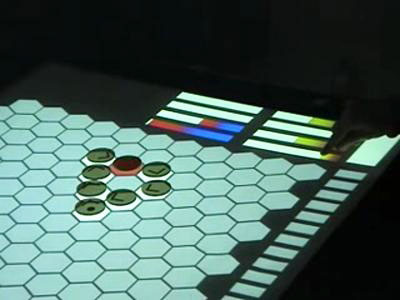
\includegraphics[scale=0.35]{1.jpg}\\
\textbf{The ReacTogon}
\end{center}

\subsection{Project Description}
Our project, branded \textit{`HEX’}, aims to emulate and extend the ReacTogon concept. Through the production of a software system that implements the harmonic table within the framework of a pattern based sequencer, we aim to provide a completely novel musical experience.

To this end, we have written a Java applet that implements the harmonic table in this way. Control is provided through the use of five counters or `operator tiles’ that are placed onto the grid, namely Play, Stop, Change, Explode and Warp. The latter four have active and inactive states which dictate whether they play a note or not during an interaction. In addition to this there are buttons and sliders to change tempo and instrument. There are also multiple layers of grids, set out in tabs, for the creation of harmony and a multi textured composition.

Our software is designed with a PC and touch screen in mind, as the tactile nature of interaction greatly lends itself to the interface. This said, the application will still run with a standard mouse and indeed, the nature of a Java applet allows portability and support for other operating systems.

\section{Background Information and Research}
\subsection{Existing Systems}
\subsubsection{Examples of Existing Software Systems}
\begin{enumerate}
\item \textbf{JR Hexatone Pro}
\begin{center}
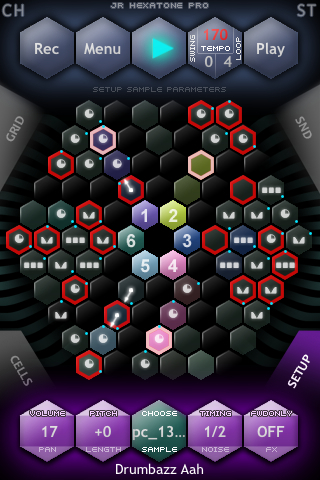
\includegraphics[scale=0.35]{2.jpg}
\end{center}
The JR Hexatone Pro is an application developed by Amidio for iOS that implements the harmonic table\cite{jrhexitunes}.  In a similar manner to the ReacTogon, tiles or `cell commands’ are placed on a circular grid of hexagons and control the nature of the sound produced. It’s unique selling point is derived from the fact that it uses `artificial intelligence and advanced randomisation algorithms’ to randomly alter the sound as the loop progresses to create a constantly changing sound. In addition to this, in place of a `start’ tile, sound is propagated from six `oscillator’ tiles at the centre of the grid and the playhead moves to one of three adjacent tiles. \cite{amidiomanual}

\item \textbf{TonePad / TonePad Pro}\\
The TonePad is another application for the iOS platform, developed by LoftLab.\cite{tonepaditunes} \\
\\
While it does not implement the harmonic table, it is based on a 16x16 matrix of notes in a pentatonic scale. To this end, it has a similar musical effect to notes played on a harmonic table. While the TonePad is simply controlled by selecting notes on the grid and has no placeable operation tiles, the ideas of playhead propagation and chain reactions are exemplified in this application. The playhead moves left to right across the grid and when a selected cell in the grid is encountered, it triggers others within a certain radius. \\
\\
A key feature of the TonePad application is it’s ability to import and export songs. Tracks can be exported as ringtones on iPhones or to m4r files. It is also possible to export song ‘code’ for sharing with others; this is integrated into the app with an ‘upload’ button. 
\end{enumerate}

\subsubsection{Examples of Existing Hardware Systems}
\begin{enumerate}
\item Tenori-On
\begin{center}
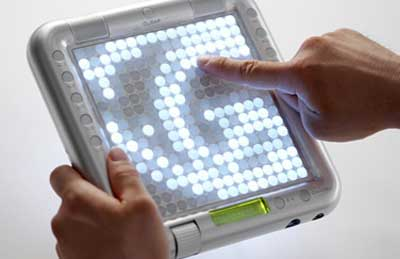
\includegraphics[scale=0.5]{3.jpg}\
\end{center}
Developed in 2005 by Japanese artist Toshio Iwai and Yu Nishibori at Yamaha\cite{tenorionwiki}, the Tenori-On is a hand-held music sequencer. Fundamentally, it is conceptually similar to the TonePad, but in hardware form and with a variety of different modes. The hardware itself consists of a 16 x 16 matrix of pressable buttons which light when activated. These buttons can act in a similar manner to the cells in the TonePad in the main sequencing mode, where highlighted cells are played when the playhead encounters them.\\
\\
In addition to this, five other modes exist such as `push mode’, which produces a continuous sound when a cell is pressed; `bounce mode’ which causes a the playhead to oscillate between the selected cell and the edge of the matrix, producing sound when `bouncing’ off the side and `grouping’ which is used to sequence patterns together.\\
\\
Each loop is composed within a layer and each layer can be thought of as `performance parts' of which there can be a total of sixteen. Different notes and instruments can be assigned to each layer and all layers can be played together in synchronisation. Each set of sixteen layers is called a block; a total of sixteen blocks can be stored and dynamically switched between in performance. In this way, musical loops and motifs can be generated and played sequentially to create a complete piece of music\cite{tenorionyamaha}.

\item \textbf{AXiS-64}
The AXiS-64 is possibly the most prevalent MIDI controller and piece of hardware that utilises the harmonic table. The equipment itself consists of the keyboard itself, composed of 192 hexagonal keys; 8 preset keys for storage of user defined keyboard configurations; 4 cursor keys, for navigating between banks; a pitch bend wheel; a modulation wheel and two rotary dials\cite{cthru}. The four analogue interfaces can be easily reprogrammed and used for any MIDI controller change.
\begin{center}
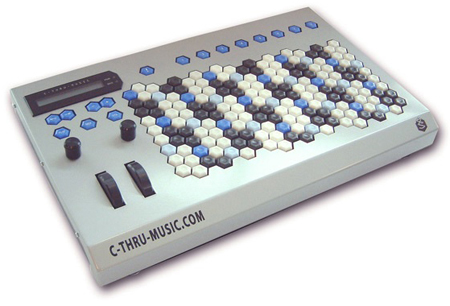
\includegraphics[scale=0.5]{4.jpg}
\end{center}
The fourth revision of the AXiS-64 firmware introduced three different keyboard modes; `single’, `split’ and `layer’.  In ‘split’ mode the keyboard is split into three 64 note keyboards; in layer it becomes one keyboard sending a signal on up to three MIDI channels when a note is played and in `single’ it acts as a single keyboard.
\end{enumerate}
\subsection{Systems Research Evaluation}
The products listed above are but a few among the systems available on the market, but each one exhibits interesting or unique characteristics that can be taken as inspiration for our project. In addition to this, there are persistent themes among all products that too will influence our designs.\\
\\
Among these common themes is the use of physical interaction as an interface between the system and the user. A considerable majority of the software systems available are for tablets or mobile devices using touch screen interfaces, with almost no standard desktop applications and only a few online hardware simulations or alternatives. This information justifies our choice of using a touch screen interface with our software.\\
\\
In addition to this, particularly interesting features of researched products that we may wish to take forward into our project include the multiple `layers' featured in the Tenori-On and the TonePad Pro's ability to export and share music and created projects. 

\subsection{Market Research}
TO BE COMPLETED
\subsection{Music Research}
\begin{center}
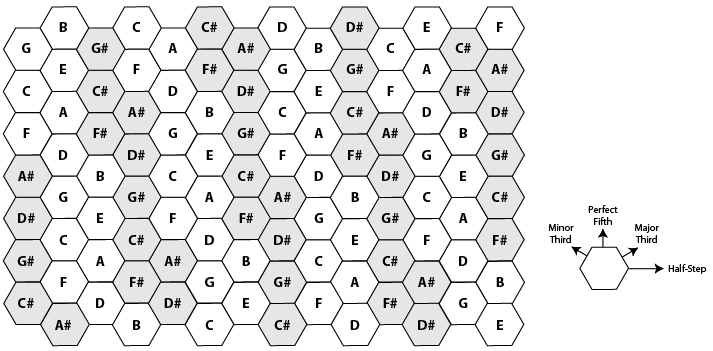
\includegraphics[scale=0.5]{5.png}
\end{center}
In musical theory, an interval is the distance between two notes or pitches. Typically, these are represented with tones and semitones, where tones are the base unit of an interval. Certain intervals appear particularly often within music and composition as they can provide key melodies. Such intervals include the perfect fifth, and major and minor thirds. These intervals, which are 7, 4 and 3 semitones above the base note respectively, make up the notes used in major and minor triads and are the intervals used in the harmonic table based on the following set of rules:\\
\\
\begin{itemize}
\item Notes ascend by an interval of a fifth on the vertical axis.
\item Notes ascend by an interval of a major third on one diagonal axis.
\item Notes ascend by an interval of a minor third on the other diagonal axis.
\end{itemize}
This layout clusters complementary notes together, for example, all the notes in the C Major chord, namely C, E and G are adjoining. Scales are played by using simple, repeated patterns that can be transposed for playing in different keys. In this way, music can be easily and quickly created.\\
\begin{center}
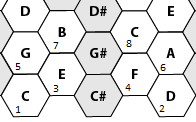
\includegraphics[scale=0.7]{scale.png}
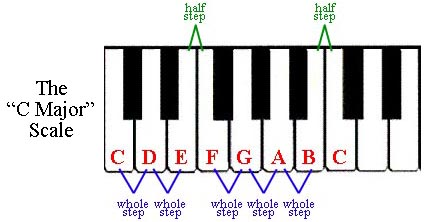
\includegraphics[scale=1.5]{scale2.jpg}
\end{center}
Above is shown a comparison of the C major scale played on a harmonic table based keyboard (left) and on a conventional piano keyboard (right). The progression is enumerated from 1 to 8.\\
\\
Scales and triads can be transposed far more easily on a harmonic keyboard than on a conventional keyboard as the basic pattern is always retained. This is shown in the G major scale below:
\begin{center}
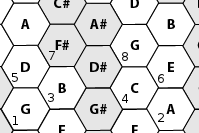
\includegraphics[scale=0.5]{scale3.png}
\end{center}
\subsection{Technical Research}
\subsubsection{MIDI}

\subsubsection{Working with Hexagons}

\section{Requirements Specification}

\subsection{Functional Requirements}

\subsection{Non-Functional Requirements}


\part{Design}
\section{Software Design}
\subsection{Code Plan}
\subsection{Key Classes and Methods}
\subsection{Keeping Time}

\section{User Interface Designs}

\part{Implementation}
\section{Implementation of Data Structures and Methods}
\subsection{Timers}
\subsection{Hexagon Cells}
\subsection{Images}

\section{Testing}
sdtujstyuj

\part{Project Meta-Comment}
hdghsghh
\section{Updates since Interim Report}

\section{Time and Planning}

\section{Problems Encountered}


\part{Conclusion}

\part{Appendices}
klujghf;kjghglkjghslkjh
\section{References}
\bibliographystyle{IEEEtran}
\bibliography{reportReferences}

\end{document}